\documentclass[fontsize=12pt, paper=a4, twoside=false, ]{scrreprt}

\usepackage{lmodern}
%\usepackage[onehalfspacing]{setspace}
\usepackage[T1]{fontenc}
\usepackage[utf8]{inputenc}
\usepackage[german]{babel}
\usepackage{microtype}% verbesserter Randausgleich
\usepackage{graphicx}
\usepackage{amsmath}
\usepackage{tikz}
\usepackage{pgfplots}
\usepgfplotslibrary{colorbrewer}
\pgfplotsset{compat = 1.15, cycle list/Set1-8} 
\usetikzlibrary{automata, positioning, arrows, colorbrewer}
\usepackage{amsfonts}
\usepackage[verbose]{placeins} 
\usepackage{longtable, needspace} %tabellen über mehrere seiten
\usepackage{listings}
\usepackage{float}
% to include sources, style
\usepackage[style=ieee,natbib=true, backend=biber]{biblatex}
\addbibresource{bib/sources.bib}


\usepgfplotslibrary{statistics}
\usepackage{pgf-pie}  
\usepackage{subcaption}
\usepackage[justification=centering, format=plain]{caption}% or e.g. [format=hang]
\usepackage{color, colortbl}
\definecolor{Gray}{HTML}{d3d3d3}
\usepackage{mathpazo} % Palatino font
\usepackage[acronym, toc]{glossaries}

% global layout
\usepackage[left=2.5cm, right=2.5cm, top=2cm, bottom=2cm]{geometry}
\setlength{\parindent}{0pt}
\widowpenalties=3 10000 10000 150
\newcommand{\cparagraph}[1]{\paragraph{#1}\mbox{}\\}
\newcommand{\cmark}{\ding{51}}%
\newcommand{\xmark}{\ding{55}}%
\setcounter{secnumdepth}{4}
\setcounter{tocdepth}{4}
\renewcommand{\baselinestretch}{1.1}
\renewcommand*{\UrlFont}{\rmfamily}
\newcommand{\mycomment}[1]{} % commenting blocks

\usepackage{listings}
% settings for links, hyperrefs
\usepackage[unicode=true,pdfusetitle,
bookmarks=true,bookmarksnumbered=false,bookmarksopen=false,
breaklinks=false,pdfborder={0 0 0},backref=false,colorlinks=false] {hyperref}
\urlstyle{sf}

\usepackage[capitalise, noabbrev]{cleveref}
\renewcommand{\lstlistingname}{Codebeispiel}% Listing -> Codebeispiel

\crefname{figure}{Abbildung}{Abbildungen}
\Crefname{figure}{Abbildung}{Abbildungen}
\crefname{listing}{Codebeispiel}{Codebeispiele}
\Crefname{listing}{Codebeispiel}{Codebeispiele}
\crefname{table}{Tabelle}{Tabellen}
\Crefname{table}{Tabelle}{Tabellen}

\makenoidxglossaries
\newacronym{llt}{LLT}{Long Lived Transaction}
\newacronym{saga-t}{T}{Transaktion}
\newacronym{saga-c}{C}{Kompensierung}

\newacronym{acid}{ACID}{Atomicity, Consistency, Isolation, Durability}
\newacronym{base}{BASE}{Basically Available, Soft State, Eventual Consistency}

\newacronym{2pc}{2PC}{Zwei-Phasen-Commit}

\begin{document}
	%\input{texes/Metadaten.tex}
	%%%%%%%%%%%%%%%%%%%%%%%%%%%%%%%%%%%%%%%%%%
% Academic Title Page
% LaTeX Template
% Version 2.0 (17/7/17)
%
% This template was downloaded from:
% http://www.LaTeXTemplates.com
%
% Original author:
% WikiBooks (LaTeX - Title Creation) with modifications by:
% Vel (vel@latextemplates.com)
%
% License:
% CC BY-NC-SA 3.0 (http://creativecommons.org/licenses/by-nc-sa/3.0/)
% 
% Instructions for using this template:
% This title page is capable of being compiled as is. This is not useful for 
% including it in another document. To do this, you have two options: 
%
	\begin{titlepage} 
		\newcommand{\HRule}{\rule{\linewidth}{0.5mm}}
		
		\center
		
		%------------------------------------------------
		%	Headings
		%------------------------------------------------
		
		\textsc{\LARGE Masterarbeit}\\[1cm] 
		
		\textsc{\Large zur Erlangung des akademischen Grades Master of Science}\\[1cm]
		
		%------------------------------------------------
		%	Title
		%------------------------------------------------
		
		\HRule\\[0.4cm]

		{\huge\bfseries Realisierung konsistenter Microservice-Systeme unter Verwendung des Saga-Patterns}\\[0.4cm]
		
		\HRule\\[1.5cm]
		
		\textsc{\Large Hochschule für Technik, Wirtschaft\\und Kultur Leipzig}\\[1.5cm] % 
		
		\begin{minipage}{0.4\textwidth}
			\begin{flushleft}
				\large
				\textit{Fakultät}\\
				\textsc{Informatik und Medien}
			\end{flushleft}
		\end{minipage}
		~
		\begin{minipage}{0.4\textwidth}
			\begin{flushright}
				\large
				\textit{Studiengang}\\
				\textsc{\large Informatik}
			\end{flushright}
		\end{minipage}
		
		\vfill
		\vfill
		
		%------------------------------------------------
		%	Author(s)
		%------------------------------------------------
		
		\begin{minipage}{0.4\textwidth}
			\begin{flushleft}
				\large
				\textit{Vorgelegt von}\\
				\textsc{Richard Werner (B.Sc.)}
			\end{flushleft}
		\end{minipage}
		~
		\begin{minipage}{0.4\textwidth}
			\begin{flushright}
				\large
				\textit{Matrikelnummer}\\
				\textsc{77353}
			\end{flushright}
		\end{minipage}
		
		
		\vfill
		
		\begin{minipage}{0.4\textwidth}
			\begin{flushleft}
				\large
				\textit{Erstprüfer}\\
				\textsc{Prof. Dr. rer. nat.\\Thomas Riechert}
			\end{flushleft}
		\end{minipage}
		~
		\begin{minipage}{0.4\textwidth}
			\begin{flushright}
				\large
				\textit{Zweitprüfer}\\
				\textsc{Johannes Elsmann (M.Sc.)}
			\end{flushright}
		\end{minipage}
		
		% If you don't want a supervisor, uncomment the two lines below and comment the code above
		%{\large\textit{Author}}\\
		%John \textsc{Smith} % Your name
		
		%------------------------------------------------
		%	Date
		%------------------------------------------------
		
		\vfill\vfill\vfill % Position the date 3/4 down the remaining page
		
		{\large\today} % Date, change the \today to a set date if you want to be precise
		
		%------------------------------------------------
		%	Logo
		%------------------------------------------------
		
		\vfill\vfill
		
\includegraphics[width=0.2\textwidth]{misc/HTWK_Zusatz_de_V_Black.jpg}\\[1cm] 
		
		%----------------------------------------------------------------------------------------
		
		\vfill % Push the date up 1/4 of the remaining page
		
	\end{titlepage}
	
	\section*{}
	\newpage
	\pagestyle{empty}
	
	\tableofcontents
	\pagebreak
	\pagenumbering{arabic}

	\section*{}
	\newpage
	\pagestyle{empty}
	
	%\chapter{Saga-Pattern}

\section{Mögliche Titel}
\begin{itemize}
	\item Realisierung konsistenter Microservice-Systeme unter Verwendung von Sagas
	\item Realisierung konsistenter Microservice-Systeme unter Verwendung des Saga-Patterns
\end{itemize}

\section{Wieso gibts das überhaupt?}
\begin{itemize}
	\item Monolithische Anwendung hat keine Probleme mit Atomarität (lokale Transaktionen sind einfach, Datenbank unterstützt Atomare Operationen)
	\item Transaktionen in verteilten Systemen: Wie kann man Atomarität erreichen? Nicht atomare Folge von Schreibe- und Sendeoperationen führen zu inkonsistenten Systemzuständen
	\item 2-Phase-Commit ist die herkömmliche Lösung, bringt aber viele meist nicht akzeptable Probleme mit sich (Chattiness, blockierend!!, wenig Durchsatz!!)
\end{itemize}

\section{Saga-Pattern} \label{Saga-Pattern-Theorie}
\begin{itemize}
	\item Kompensations-Mechanismus für verteilte Transaktionen (Was passiert, wenn eine Operation fehlschlägt? Timeout?)
	\item Sicherstellung der Konsistenz des Systemzustands (Verteilte Transaktion sollte ein Übergang zwischen zwei konsistenten Zuständen sein)
	\item Orchestration und Choreographie
	\item Idempotenz
	\item Synchron und Asynchrone Verfahren
	\item ACID und BASE
\end{itemize}

\section{Design eines Microservice-Systems unter Verwendung des Saga-Patterns}
\begin{itemize}
	\item Verwenden der Punkte aus \ref{Saga-Pattern-Theorie}
	\item Verfolgen unterschiedlicher Ansätze (Orchestration und Choreographie)
	\item Bewertung und Vergleich der Designs
\end{itemize}

\section{Problemstellung}
\par Die Realisierung von Transaktionen in verteilten Systemen bringt viele Probleme mit sich. Das Saga-Pattern ist eine Möglichkeit, diese Probleme im Kontext von Microservices zu bewältigen. 

\par Im Rahmen der Masterarbeit soll das Saga-Pattern vorgestellt werden und die mit dem Systemdesign verbundenen Überlegungen anhand eines zu Beginn definierten Fallbeispiels erläutert werden. 

\par Es sind zwei Architekturen mit dazugehörigem Design unter Verwendung des Choreographie- und des Orchestrationsansatzes zu entwerfen und zu bewerten und zu vergleichen. Die Bewertung und der Vergleich sind vorrangig unter dem Blickwinkel der Systemkonsistenz durchzuführen. 
	
	\chapter{Einleitung}

Moderne Anwendungen bestehen häufig aus mehreren individuellen Komponenten, die an der Lösung einer gemeinsamen Aufgabe beteiligt sind. Dabei besteht die Aufgabe einer Komponente oft darin, eine Anfrage entgegenzunehmen, bestimmte Bedingungen zu prüfen, die Daten zu transformieren, in einer Datenbank zu speichern und auf den Aufrufer mit einem Ergebnis zu antworten. Solche modularen Komponenten tauchen besonders im Architekturstil der Microservices auf. Ein Ziel der Modularisierung ist eine möglichst geringe Bindung der Services, damit die Komplexität innerhalb einer Komponente gering gehalten wird und falls notwendig durch eine andere Komponente ausgetauscht werden kann. Deshalb arbeiten Microservices oft mit einer eigenen Datenbank, die nur von diesem Service erreichbar ist. 

Aufgrund der Verteilung der Daten über mehrere Datenbanken entstehen neue Herausforderungen, die das System bewältigen muss. Besonders die Verwendung von transaktionellen Operationen stellt die Herausforderung der verteilten Transaktionen. Die Mechanismen des Transaktionsinterfaces von \acrshort{acid}-Transaktionen einer relationalen Datenbank funktionieren nur dann, wenn alle auszuführenden Operationen in einem Transaktionskontextes ausgeführt werden. Prozesse, die atomare Veränderungen in mehreren Datenbanken bewirken sollen, werden als verteilte Transaktionen bezeichnet. 

Commitprotokolle wie etwa der \acrfull{2pc} stellen eine mögliche Implementierung verteilter Transaktionen, die ACID-Eigenschaften gewährleisten können. Dabei werden jedoch die betroffenen Ressourcen blockiert, was zu einem geringen Durchsatz führen kann. In Fällen, die unter keinen Umständen Inkonsistenzen gewährleisten können, ist dies eine praktikable Lösung. In Systemen, die für einen Zeitraum einen inkonsistenten Systemzustand annehmen dürfen, können die Änderungen sequentiell prozessiert werden. Dies verspricht eine höhere Verfügbarkeit und höheren Durchsatz. Der Begriff der schlussendlichen Konsistenz (\textit{Eventual Consistency}) beschreibt dieses Verhalten. 

\section{Fragestellung}
Diese Arbeit verwendet das von \citeauthor{GarciaMolina.1987} vorgeschlagene Muster des Saga-Patterns im Kontext eines verteilten Systems. Das Muster verspricht atomares Verhalten mehrere Operationen in einer sequentiellen Ausführung. Dies erlaubt die Verwendung des Musters im Kontext verteilter Transaktionen. 

Der zentrale Punkt des Musters befasst sich mit der Behandlung von Fehlern während der Transaktion. Es soll untersucht werden, ob Netzwerkausfälle in diese Fehlerbehandlung integrierbar sind.

\section{Aufbau dieser Arbeit}
\cref{chapter_grundlagen} befasst sich mit dem Begriff der Transaktion. Dabei werden damit verbundene Konzepte in zentralisierten und verteilten Systemen vorgestellt.

In \cref{chapter_sagapattern} wird \citeauthor{GarciaMolina.1987}s Arbeit \citetitle{GarciaMolina.1987} referenziert. Außerdem wird das darin definierte Entwicklungsmuster in den Kontext verteilter Systeme eingeordnet. Zusätzlich wird eine Formalisierung vorgenommen, die die Beschreibung von mittels Saga-Pattern implementierter Transaktionen erlaubt. 

Die Vermutung, dass die Fehlerbehandlung des Saga-Patterns Netzwerkausfälle integrieren kann, soll in einem Versuch überprüft werden. \cref{chapter_versuchsvorbereitung} bereitet den durchzuführenden Versuch vor. In diesem Kapitel wird das zu entwerfende System definiert indem ein imaginärer Geschäftsprozess definiert wird, der mittels Saga-Pattern umgesetzt werden soll. Es werden Metriken definiert, die der Beantwortung der These dienen sollen. Die Durchführung des Versuchs wird in \cref{chapter_versuchsdurchführung} erläutert. Die im Versuch gesammelten Messwerte, Ergebnisse und Zusammenhänge werden in \cref{chapter_versuchsergebnis} dargestellt. Die These und die dazugehörigen Leitfragen werden in diesem Kapitel beantwortet. 












	
	\chapter{Grundlagen}

% Hier kommen alle Begriffsdefinitionen rein, die isoliert erklärt werden können
%Um das in dieser Arbeit betrachtete Saga-Pattern zu verstehen, sollen zuerst einige Grundlagen erläutert werden. Besonders die im Titel der Arbeit enthaltenen Begriffe \textit{System} und \textit{Konsistenz} sollen in diesem Abschnitt erläutert werden. 
%
%\subsection{System allgemein}
%Ein System beschreibt einen abgegrenzten Bereich der objektiven Realität. Außerhalb dieses Bereichs liegt die Umgebung, die somit nicht zum System gehört. Zwischen des Systems und seiner Umgebung befindet sich der Systemrand. 
%
%\subsection{System in der Softwareentwicklung}
%In der Softwareentwicklung besteht ein System aus einer Menge miteinander interagierenden Softwarekomponenten. Diese Komponenten arbeiten an einem gemeinsamen Ziel. Neben der Software und deren Quellcode gehören auch Nutzerhandbücher, Tests, Bestandteile für die Instandhaltung sowie Spezifikationen und Konzepte zum System. 
%
%\subsection{Zustand von Systemen}
%Ein Softwaresystem befindet sich zu jedem Zeitpunkt in einem Zustand. Der Wechsel eines Zustands ist die Folge von Nutzerinteraktionen und festgelegten Routinen. Damit das System reibungslos funktionieren kann, darf es nur zwischen gültigen Zuständen wechseln. % TODO Was ist ein gültiger Zustand





% Hier kommen Ansätze rein, die in verteilten Systemen der Konsistenz dienen
\input{texes/ChapterGrundlagen/Lösungsstrategien.tex}

	
	
	\chapter{Das Saga Pattern} \label{chapter_sagapattern}

\input{texes/ChapterSaga/PaperÜberblick.tex}

\input{texes/ChapterSaga/PaperFürVerteilteTransaktionen.tex}

\section{Bestandteile des Musters}
\subsection{Funktionsweise}
Eine Operation ist im Saga-Pattern eine lokale Transaktion, die in sich geschlossen ist und die ACID-Eigenschaft erfüllen muss. Für eine solche Operation wird gleichzeitig eine Schnittstelle angeboten, die die Veränderungen rückgängig macht. Somit besteht die Möglichkeit eine Operation zu neutralisieren. Es wird also die Anforderung an den Entwickler gestellt, für jede angebotene Operation eine Umkehroperation bereitzustellen, die selbst eine lokale Transaktion darstellt. 
Im Paper werden lokale Transaktionen, die eine Operation der Transaktion darstellen, als Ts bezeichnet. Die dazugehörigen lokalen Transaktionen werden als Cs bezeichnet. 

Zur Ausführung der LLT werden die Ts sequentiell aufgerufen (im Gegensatz zum gleichzeitig ausgelösten Transaktionsstart im \acrshort{2pc}). Tritt bei der Ausführung eines Ts ein Fehler auf, können alle bereits ausgeführten Operationen in ihren Ursprungszustand zurückgesetzt werden, indem in der umgekehrten Reihenfolge die notwendigen Cs aufgerufen werden. Im Fehlerfall wird der Ausgangszustand in allen Services wiederhergestellt und die Atomarität der Transaktion ist gewährleistet. Sind alle Operationen erfolgreich, wird nach Ausführung aller Ts der Endzustand erreicht und die Transaktion hat einen neuen Zustand hergestellt. Sowohl im erfolgreichen als auch im kompensierten Endzustand ist die Konsistenz gewahrt.

\subsection{Transaktionsteilnehmer}
Die verteilte Saga setzt voraus, dass die Operation nicht zentralisiert innerhalb eines geschlossenen Systems umgesetzt werden kann. Die Teiloperationen sind über mehrere Services verteilt. Diese Services werden als Teilnehmerservice bezeichnet. Es liegt in der Verantwortung der Entwickler des entsprechenden Teilnehmerservices, die Teiloperation über eine Schnittstelle anzubieten und korrekt zu implementieren. Darunter fällt auch die Implementierung der dazugehörigen Kompensierung. Dabei verwaltet jeder Service seine eigenen Daten in einer eigenen Datenbank. Dieses Muster nennt sich Database-per-Service-Pattern und ist sehr verbreitet in der Entwicklung von Microservices \cite{microservices.io.12.01.2024}. 

\subsection{Formulieren der Kompensierungstransaktionen}
Die einzelnen Operationen, die ausgeführt werden müssen, müssen kompensiert werden können. Eine solches T wird als lokale Transaktion betrachtet, die in einem anderen Service stattfindet. Der Nebeneffekt der Transaktion ist häufig eine Veränderung in der Datenbank. Es wird nun betrachtet, welche verschiedenen Effekte T in der Datenbank haben kann und welchen Effekt das entsprechende C haben muss.

\paragraph*{Insert} \mbox{}\\
Äußert sich der Effekt von T in einem Insert, dann ist der kompensierende Effekt von C ein Delete. Alternativ kann ein Soft-Delete implementiert werden, der den Datensatz als ungültig markiert.

\paragraph*{Update} \mbox{}\\
Beim Kompensieren von Updates wird zwischen idempotenten und nicht-idempotenten Updates unterschieden. Zur Veranschaulichung sollen die in \cref{lst:sql-idempotent-update} und \cref{lst:sql-nicht-idempotent-update} dargestellten SQL-Statements betrachtet werden. 

\begin{figure}[!htbp]
\centering
\begin{minipage}{.42\textwidth}
	\begin{lstlisting}[language=SQL, breaklines=true, tabsize=2, showstringspaces=false, frame=single, basicstyle=\small, label = {lst:sql-idempotent-update}, caption={SQL Skript für ein idempotentes Update}, captionpos=b]
update stock 
set amount = 10
where id = 42 and ...
	\end{lstlisting}
\end{minipage}
\hspace{1.5cm}
\begin{minipage}{.42\textwidth}
	\begin{lstlisting}[language=SQL, breaklines=true, tabsize=2, showstringspaces=false, frame=single, basicstyle=\small, label = {lst:sql-nicht-idempotent-update}, caption={SQL Skript für ein nicht-idempotentes Update}, captionpos=b]
update stock 
set amount = amount - 1
where id = 42 and ...
	\end{lstlisting}
\end{minipage}
\end{figure}
\FloatBarrier

In \cref{lst:sql-idempotent-update} wird ein Update-Statement ausgeführt, welches den entsprechenden Wert \textit{amount} auf 10 setzt. Dabei geht die Information des vorherigen Zustands verloren. Eine Kompensierung ist hier nur möglich, indem eine zusätzliche History-Tabelle verwendet wird. 

In \cref{lst:sql-nicht-idempotent-update} wird ein Update-Statement ausgeführt, welches den entprechenden Wert \textit{amount} um 1 verringert. Um dieses Update zu kompensieren, muss der alte Wert nicht bekannt sein, wenn die LLT Kenntnis von dem Wert der Änderung hat. Es kann eine Kompensierung in Form einer Addition um den selben Wert durchgeführt werden. 

\paragraph*{Delete} \mbox{}\\
Das Löschen eines Datensätzes kann nur kompensiert werden, wenn der gesamte Eintrag vor dem Löschen gespeichert wurde (History-Tabelle). Falls T nur ein Soft-Delete ausgelöst hat, kann die Markierung der Ungültigkeit zur Kompensierung aufgehoben werden.

\paragraph*{Ts ohne Nebeneffekte} \mbox{}\\
Es ist möglich, dass ein T eine Operation durchführt, die zu keiner Nebenwirkung führt. Beispielsweise kann dies der Aufruf einer Schnittstelle sein, um einen Wert zu validieren. In diesem Fall muss die Kompensierung nicht implementiert werden. 

Es ist hervorzuheben, dass der Effekt eines Ts neben Änderungen in der Datenbank oder Aufrufe von anderen Schnittstellen auch reale Geschäftsprozesse auslösen können. Ein solcher Prozess kann unter Umständen nicht kompensierbar sein. Hier kann auch weiter differenziert werden. 

\paragraph*{Nicht kompensierbare Ts} \mbox{}\\
Ist der Effekt von T die Versendung eines Briefs, so kann diese Versendung nicht kompensiert werden. Ein Folgebrief kann jedoch als Kompensierung angesehen werden, die den ausgelösten Effekt neutralisiert. Im Folgebrief können beispielsweise Anweisungen stehen, die den Empfänger informieren, dass der vorherige Brief als ungültig angesehen werden kann. Der Effekt von T kann hier als kompensiert angesehen werden. 

Es gibt jedoch auch Effekte, die nicht kompensierbar sind und im Scheitern einer Saga resultieren. In solchen Fällen kann das System in einen inkonsistenten Zustand überführt werden. Dieses Verhalten tritt immer dann auf, wenn der Effekt einer Transaktion in einer endgültigen Aktion resultiert. \citeauthor{GarciaMolina.1987} nennen als Beispiel für ein nicht kompensierbares T das Starten einer Rakete \cite[p.257]{GarciaMolina.1987}.

\subsection{Komponenten des Saga-Patterns}
\citeauthor{GarciaMolina.1987} nennt folgende Komponenten als Grundbausteine des Saga-Patterns:
\begin{itemize}
	\item Transaktionen und Kompensierungen
	\item Transaction Execution Component
	\item Saga Execution Component
\end{itemize}

\paragraph*{Transaktionen und Kompensierungen} \mbox{} \\
Das Aufteilen einer Transaktion in die entsprechenden Teiltransaktionen sowie das Verhalten im Falle eines Fehlers wurden bereits in erläutert. Nach Übertragung des Musters auf ein verteiltes System finden diese Ts und Cs innerhalb eines Teilnehmerservices statt. 

\paragraph*{Transaction Execution Component} \mbox{} \\
Die \acrfull{tec} wird beschrieben als eine Komponente, die die Ausführung der zu einer Teiltransaktion gehörenden Aktionen ausführt. Eine an die \acrshort{tec} gestellte Anfrage für die Ausführung einer Teiltransaktion wird atomar verarbeitet. In der verteilten Implementierung einer Saga befindet sich die \acrshort{tec} innerhalb eines jeden Teilnehmerservices. Auf Anfrage wird ein T oder ein C ausgeführt. Alle dafür erforderlichen Datenbankoperationen bestehen innerhalb eines herkömmlichen ACID-Transaktionskontexts. 

\paragraph*{Saga Execution Component} \mbox{} \\
Die \acrfull{sec} ist die äußerste Schicht aller Sagakomponenten. Sie ist zuständig für die Ausführung der Saga. Dazu gehört das sequentielle Aufrufen aller Teiltransaktionen und die Reaktion mit Kompensierungstransaktionen im Falle von Fehlschlägen. Eine weitere Aufgabe der \acrshort{sec} ist das Neustarten der Saga im Falle eines Absturzes. 

Die \acrshort{sec} verwendet ein Transaktionslog, um den Prozessablauf zu steuern. Dieses Log enthält für jede Saga die Liste an ausgeführten Schritten. Eine Liste der vergangenen Werte kann auch Bestandteil des Logs sein, damit im Falle von Kompensierungen der ursprüngliche Stand gesetzt werden kann. 

%\section{Bestandteile des Musters}

Ein Saga-System 

\subsection{Systembestandteile}
Zunächst soll dargestellt werden, aus welchen Systembestandteilen eine per Saga-Pattern umgesetzte LLT besteht. Es gibt mehrere Teilnehmerservices, die angebunden werden müssen, um die zur LLT gehörenden Transaktionen auszuführen. 


\subsection{Aufteilen der LLT}
Aufteilung der LLT in Ts und Kompensierende Cs

\subsection{Systemkomponenten}
SEC
TEC
Menge von Ts





\section{Formalisierung eines Saga-Zustandsautomaten als DEA} \label{sec_saga_formalisierung_dea}
%TODO Abkürzung DEA
\subsection{Formale Darstellung eines DEA}
Der Prozessablauf einer Saga kann als detemernistischer endlicher Automat angesehen werden. Ein DEA wird formal dargestellt als Tupel mit folgenden Elementen:
\begin{itemize}
	\item $Q$: Zustandsmenge
	\item $\Sigma$: endliches Eingabealphabet
	\item $\delta: Q \times \sum \rightarrow Q$: Übergangsrelation 
	\item $q_0 \in Q$: Startzustand
	\item $F \subseteq Q$: Menge an akzeptierenden Zuständen
\end{itemize}

\subsection{Saga als formale Sprache}
%TODO Deterministisch, totale Funktion, Angenommene Sprache, referenz vorheriges subsubsection
Im vorherigen Abschnitt wurde die Saga Execution Component definiert als ein Tupel aus Transaktionslog und Zustandsautomat. Nun soll dieses Tupel in einen DEA überführt werden. Ein solcher DEA $A_{Saga}$ akzeptiert die Sprache $L_{Saga}$, die alle gültigen Wörter enthält, die eine Saga darstellen.

Das Eintabealphabet $\Sigma$ ist die Menge aller Elemente, die im Transaktionslog auftauchen können. Somit kann jedes Transaktionslog als Eingabewort aufgefasst werden. 

Somit ist die von $A_{Saga}$ akzeptierte Sprache $L_{Saga} = L(A_{Saga})$: \\

\begin{center}
	$\forall w \in \Sigma^{\star}: w \in L(A_{Saga}) \iff w \in L_{Saga}$
\end{center}

% TODO prüfen von hier. Passt das auf 
\subsection{Überführung einer Saga in einen DEA}
Um eine Saga in einen DEA überführen zu können, müssen zuerst einige Definitionen vorgenommen werden. Die Unterscheidung zwischen Ts und Cs wird im Modell eines Zustandsautomaten per Zustand ausgedrückt. Es muss also eine Abstrahierung vorgenommen werden, die Ts und Cs vereinigt. Diese Abstrahierung wird im Folgenden als $Aktion\ A$ bezeichnet. Eine solche Aktion $a_n$ wird immer im entsprechenden Zustsand $q_n \in Q$ ausgeführt. In der folgenden Erläuterung kann die Zustandsmenge $Q$ mit der Menge $T \cup C$ gleichgesetzt werden.

Das Eingabealphabet $\Sigma$ drückt aus, welche möglichen Ergebnisse eine Aktion haben kann. Eine Aktion kann einerseits ein Aufruf einer externen Schnittstelle sein. Die Antwort dieser Schnittstelle kann das Ergebnis in unterschiedlichen Formen ausdrücken. Das können beispielsweise folgende Ausdrucksformen sein:
\begin{itemize}
	\item Http-Statuscode
	\item Custom Http-Responsebody
\end{itemize}
Diese sind üblicherweise in einer Schnittstellendefinition aufgelistet. Im Folgenden wird davon ausgegangen, dass alle möglichen Antworten einer Http-Schnittstelle per Http-Statuscode ausgedrückt werden. Es wird ein Typ definiert, der für jede Aktion alle möglichen Http-Statuscodes enthält: 

\begin{center}
	$API-Ergebnis\ AE \in \{tn_{200}, tn_{201}, tn_{400}, tn+1_{200}, tn+1_{400}, tn+1_{409}, ...\}$. 
\end{center}

Eine Aktion kann neben dem Aufruf einer Schnittstelle eine interne Verarbeitung sein. Das könnte beispielsweise eine Prüfung auf Vorhandensein eines Feldes in einer vorangegangenen Schnittstellenantwort sein. Eine solche Aktion wird definiert:

\begin{center}
	$Internes\ Prozessergebnis\ IPE \in \{tn_{Success}, tn_{Failure}, tn+1_{Success}, tn+1_{Failure}, ...\}$.
\end{center}

Ein Ergebnis einer Aktion wird also definiert als:

\begin{center}
	$Ergebnis\ E = AE \cup IPE$.
\end{center}

Das Eingabealphabet beinhaltet Elemente aus dem Ergebnistyp: 

\begin{center}
	$\Sigma = Ergebnis$.
\end{center}

Ein Übergang von einem Zustand in den Folgezustand drückt somit aus, dass die Saga eine Aktion ausgeführt hat und dem Ergebnis entsprechend einen Zustandswechsel durchgeführt hat. 

Der Startzustand $q_0$ ist die erste auszuführende Transaktion. 

Ein Endzustand $q_{f1}$ wird erreicht, nachdem die letzte auszuführende Transaktion erfolgreich beendet wurde. Ein weiterer Endzustand $q_{f2}$ wird erreicht, nachdem die letzte Kompensierung erfolgreich beendet wurde. Der letzte Endzustand $q_{f3}$ wird erreicht, nachdem die erste Kompensierung erfolglos beendet wurde.
% TODO vielleicht qf3 nicht als akzeptierenden Zustand markieren: beeinflusst, welche Sprache der DEA akzeptiert

\paragraph*{Konfiguration}\mbox{}\\
% TODO https://www.cs.uni-potsdam.de/ti/lehre/06-Theorie-I/slides/slides-2.1.pdf
Die Ausführung eines DEA kann mittels Konfigurationen dargestellt werden. Eine Konfiguration $K$ ist definiert als: 

\begin{center}
	$K = (q, w) \in Q \times \Sigma^{\star}$
\end{center}

Der Automat wechselt in einen Folgezustand, indem er ein Element aus dem Eingabewort abarbeitet und eine passende Übergangsrelation in $\delta$ findet. Somit gilt:

\begin{center}
	$q1, q2 \in Q \land u \in \Sigma \land v \in \Sigma^{\star}: (q_{1}, u \circ v)\vdash (q_{2}, v) \implies \delta(q_{1}, u) = q_{2}$
\end{center}

Außerdem können mehrere Konfigurationsübergänge mittels $\vdash^{\star}$ dargestellt werden:

\begin{center}
	$K_1 \vdash^{\star} K_2 \implies \ K_1 = K_2 \lor \exists K: K_1 \vdash K \land K \vdash^{\star} K_2$
\end{center}

\subsection{Betrachtung des Zustands nach Erfolg/Misserfolg}\label{subsubsection_dea_simple}
Der Zustand des Systems soll nun in folgenden Fällen betrachtet werden:
\begin{enumerate}%TODO Anpassen an Paragraphenüberschriften
	\item Erfolgreicher Ablauf einer Saga
	\item Scheitern der Saga nach n Schritten
	\item Scheitern der Saga nach n Schritten und Scheitern der Kompensierung nach m Schritten
\end{enumerate}

Die Ausführung der Saga als DEA soll an folgendem Beispiel illustriert werden:

$Saga = (Q, \Sigma, \delta, q_0, F)$ mit
\begin{align*}
	Q &= \{q_{t1}, q_{t2}, q_{t3}, q_{c1}, q_{c2}, q_{c3}, q_{f1}, q_{f2}, q_{f3}\}\\
	\Sigma &= \{t1_{200}, t1_{400}, t2_{Success}, t2_{Failure}, t3_{200}, t3_{400}, c1_{200}, c1_{400}, c2_{Sucess}, c2_{Failure}, c3_{200}, c3_{400}\}\\
	\delta &= \{((q_{t1}, t1_{200}), q_{t2}), 
	((q_{t2}, t2_{Sucess}), q_{t3}), 
	((q_{t3}, t3_{200}), q_{f1}), 
	((q_{t1}, t1_{400}), q_{f2}), \\
	&((q_{t2}, t2_{Failure}), q_{c1}), 
	((q_{t3}, t3_{400}), q_{c2}), 
	((q_{c1}, c1_{200}), q_{f2}), 
	((q_{c2}, c2_{Sucess}), q_{c1}),\\ 
	&((q_{c3}, c3_{200}), q_{c2}), 
	((q_{c1}, c1_{400}), q_{f3}), 
	((q_{c2}, c2_{Failure}), q_{f3}), 
	((q_{c3}, c3_{Failure}), q_{f3})\} \\
	q_0 &= q_{t1}\\
	F &= \{q_{f1}, q_{f2}, q_{f3}\}
\end{align*}


\begin{figure}[ht!]
	\centering
	\begin{tikzpicture}[->,>=stealth',shorten >=1pt,auto,node distance=2.5cm, semithick]
		\node [state, initial] 		(qt1) 					{$q_{t1}$};
		\node [state] 				(qt2) [right of=qt1] 	{$q_{t2}$};
		\node [state] 				(qt3) [right of=qt2] 	{$q_{t3}$};
		
		\node [state] 				(qc1) [below of=qt2] 	{$q_{c1}$};
		\node [state] 				(qc2) [right of=qc1] 	{$q_{c2}$};
		\node [state] 				(qc3) [right of=qc2] 	{$q_{c3}$};
		
		\node [state, accepting] 	(qf1) [right of=qt3] 	{$q_{f1}$};
		\node [state, accepting] 	(qf2) [left of=qc1] 	{$q_{f2}$};
		\node [state, accepting] 	(qf3) [below of=qc2] 	{$q_{f3}$};
		
		\path (qt1) 	edge					node 		{$t1_{200}$}		(qt2)
		edge					node		{$t1_{400}$}		(qf2)
		(qt2)		edge					node		{$t2_{Success}$}	(qt3)
		edge					node		{$t2_{Failure}$}	(qc1)
		(qt3)		edge					node		{$t3_{200}$}		(qf1)
		edge					node		{$t3_{400}$}		(qc2)
		(qc1)		edge					node		{$c1_{200}$}		(qf2)
		edge	[bend right]	node		{$c1_{400}$}		(qf3)
		(qc2)		edge					node		{$c2_{Success}$}	(qc1)
		edge					node		{$c2_{Failure}$}	(qf3)
		(qc3)		edge					node		{$c3_{200}$}		(qc2)
		edge	[bend left]		node		{$c3_{400}$}		(qf3);
	\end{tikzpicture}
	\caption{Darstellung einer Saga als Deterministischen endlichen Automaten}
\end{figure}
\FloatBarrier

\paragraph*{Endzustand $q_{f1}$} \mbox{}\\
Im Folgenden wird davon ausgegangen, dass die Aktionen der Zustände $q_{t1}$, $q_{t2}$ und $q_{t3}$ in einem erfolgreichen Ergebnis resultieren. Somit wird am Ende der Endzustand $q_{f1}$ erreicht. Dieser Zustand drückt einen erfolgreichen Durchlauf einer Saga aus. Das Eingabewort $e_1 \in \Sigma^{\star}$ ist $t1_{200} \circ t2_{Success} \circ t3_{200} \circ \#$.

Die Konfigurationsübergänge für $e_1$ sind:

\begin{align*}
	(q_{t1}, t1_{200} \circ t2_{Success} \circ t3_{200} \circ \#)\\
	\vdash(q_{t2}, t2_{Success} \circ t3_{200} \circ \#)\\
	\vdash (q_{t3}, t3_{200} \circ \#)  \\
	\vdash (q_{f1}, \#)
\end{align*}


\paragraph*{Endzustand $q_{f2}$} \mbox{}\\
Es wird nun davon ausgegangen, dass bei der Aktion im Zustand $q_{t3}$ ein Ergebnis $t3_{400}$ erfolgt. Ein solches Ergebnis führt dazu, dass der Zustand $q_{c2}$ erreicht wird. Hier wird davon ausgegangen, dass die Aktionen $q_{c2}$ und $q_{c1}$ erfolgreiche Ergebnisse haben. Das Eingabewort $e_2 \in \Sigma^{\star}$ ist $t1_{200} \circ t2_{Success} \circ t3_{400} \circ c2_{Success} \circ c1_{200}$.

Die Konfigurationsübergänge für $e_2$ sind:

\begin{align*}
	(q_{t1}, t1_{200} \circ t2_{Success} \circ t3_{400} \circ c2_{Success} \circ c1_{200} \circ \#)\\
	\vdash (q_{t2}, t2_{Success} \circ t3_{400} \circ c2_{Success} \circ c1_{200} \circ \#))\\
	\vdash (q_{t3}, t3_{400} \circ c2_{Success} \circ c1_{200} \circ \#))\\
	\vdash (q_{c2}, c2_{Success} \circ c1_{200} \circ \#))\\
	\vdash (q_{c1}, c1_{200} \circ \#))\\
	\vdash (q_{f2}, \#))
\end{align*}


\paragraph*{Endzustand $q_{f3}$} \mbox{}\\
Zuletzt soll der Zustand $q_{f3}$ betrachtet werden. Dafür soll die Aktion in $q_{t3}$ das Ergebnis $t3_{400}$ haben. Danach schlägt die Aktion $q_{c2}$ fehl und liefert das Ergebnis $c2_{Failure}$. Das Eingabewort $e_3 \in \Sigma^{\star}$ ist $t1_{200} \circ t2_{Success} \circ t3_{400} \circ c2_{Failure} \circ \#$.

Die Konfigurationsübergänge für $e_3$ sind:

\begin{align*}
	(q_{t1}, t1_{200} \circ t2_{Success} \circ t3_{400} \circ c2_{Failure} \circ \#) \\
	\vdash (q_{t2}, t2_{Success} \circ t3_{400} \circ c2_{Failure} \circ \#) \\
	\vdash (q_{t3}, t3_{400} \circ c2_{Failure} \circ \#) \\
	\vdash (q_{c2}, c2_{Failure} \circ \#) \\
	\vdash (q_{f3}, \#) \\
\end{align*}

\subsection{Recovery-Mechanismen} %TODO klare Definition einfügen und hier referenzieren, Zitat Paper Saga 1987
Eine Saga, die in der Ausführung einer Transaktion fehlschlägt, wechselt nach der Definition in die entsprechende Kompensierung und versucht, alle bis dahin ausgeführten Transaktionen zu kompensieren. Somit wird der Anfangszustand des Systems wiederhergestellt. Dieses Verhalten wird als Backward-Recovery bezeichnet. 

Neben der Backward Recovery wird ein weiteres Verhalten vorgeschlagen, welches Forward-Recovery genannt wird. Das Ziel der Forward Recovery ist es, seltener in einem erfolglosen Endzustand zu gelangen. Im Modell der hier aufgestellten DEA-Saga sind das Zustände $q_{f2}$ und $q_{f3}$. Um dies zu erreichen, werden Save-Points definiert. Ein Save-Point stellt einen Zustand dar, von dem bei einem Systemabsturz oder einem erfolglosen Ergebnis die Ausführung weitergeführt werden kann. Es wird im Fehlerfall Backward-Recovery bis zum nächsten Save-Point ausgeführt. Wird dieser erreicht, werden alle noch fehlenden Ts ausgeführt, um zum erfolgreichen Endzustand zu gelangen. Das bedeutet, dass von der Kompensierungskette zurück auf die Transaktionskette gesprungen wird.


\paragraph*{Backward Recovery}\mbox{}\\
 %TODO referenz DEA
Der DEA einer Saga, die Backward-Recovery implementiert, ist im vorherigen Abschnitt beschrieben.

\paragraph*{Forward Recovery} \mbox{}\\
% TODO referenz DEA
Forward-Recovery ist auf verschiedenen Wegen erreichbar. Der erste Ansatz beinhaltet die Verwendung eines Save-Points. Der DEA aus Abschnitt soll um einen Checkpoint und Forward Recovery ergänzt werden. Es wird ein weiterer Zustand eingeführt, der nach erfolgreichem Ergebnis von $q_{t1}$ erreicht wird. Der Checkpoint wird hier dargestellt als ein interner Prozessschritt $q_{sp1}$ und hat somit die möglichen Ergebnisse $\in \{sp1_{Success}, sp1_{Failure}\}$. Es ist zu sehen, dass dieser DEA eine mögliche Endlosschleift zulässt. Wenn $q_{sp1}$ erreicht wird und in $q_{t2}$ oder $q_{t3}$ immer ein erfolgloses Ergebnis auftritt, darf im Zustand $qsp1$ nur endlich oft der Übergang $sp1_{Success}$ gewählt werden. 

Die Funktion $f$ die in $q_{sp1}$ ein internes Prozessergebnis $IPE$ berechnet, sieht so aus:
\begin{flalign*}
	&f: \mathbb{N} \rightarrow IE &&\\
	&maxSavepointExecutionCount \in \mathbb{N}: Anzahl\ des\ Erreichens\ von\ q_{sp1}\ während\ &\\ 
	&der\ Ausführung\ der\ Saga 
\end{flalign*}

\begin{equation*}
	f(x) = 
	\begin{cases}
		IE_{Success}, x < maxSavepointExecutionCount\\
		IE_{Failure}, else
	\end{cases}
\end{equation*}

Die Anzahl an Ausführungen beginnend bei $q_{t2}$ ist begrenzt. Es wird also solange Forward Recovery versucht, bis die Saga erfolgreich ist oder das Oberlimit $maxSavepointExecutionCount$ erreicht wird. Wenn dieses Oberlimit erreicht ist, wird die Forward Recovery aufgegeben und in den Zustand $q_{c1}$ gewechselt.


\begin{figure}[ht!]
	\centering
	\begin{tikzpicture}[->,>=stealth',shorten >=1pt,auto,node distance=2.5cm, semithick]
		\node [state, initial] 		(qt1) 					{$q_{t1}$};
		\node [state]				(qsp1)[below right=2cm and 3cm of qt1]	{$q_{sp1}$};
		\node [state] 				(qt2) [above right=2cm and 3cm of qsp1] 	{$q_{t2}$};
		\node [state] 				(qt3) [right=2cm of qt2] 	{$q_{t3}$};
		
		\node [state] 				(qc1) [below left=2cm and 3cm of qsp1]{$q_{c1}$};
		\node [state] 				(qc2) [below right=2cm and 3cm of qsp1] 	{$q_{c2}$};
		
		\node [state, accepting] 	(qf1) [right of=qt3] 	{$q_{f1}$};
		\node [state, accepting] 	(qf2) [left of=qc1] 	{$q_{f2}$};
		\node [state, accepting] 	(qf3) [below of=qc2] 	{$q_{f3}$};
		
		\path (qt1) 	edge	[bend right]	node 		{$t1_{200}$}		(qsp1)
		edge					node		{$t1_{400}$}		(qf2)
		(qt2)		edge					node		{$t2_{Success}$}	(qt3)
		edge	[bend left]		node		{$t2_{Failure}$}	(qsp1)
		(qt3)		edge					node		{$t3_{200}$}		(qf1)
		edge					node		{$t3_{400}$}		(qc2)
		(qc1)		edge					node		{$c1_{200}$}		(qf2)
		edge	[bend right]	node		{$c1_{400}$}		(qf3)
		(qc2)		edge	[bend right]	node		{$c2_{Success}$}	(qsp1)
		edge					node		{$c2_{Failure}$}	(qf3)
		(qsp1) 	edge	[bend left]		node		{$sp1_{Success}$}	(qt2)
		edge	[bend right]	node		{$sp1_{Failure}$}	(qc1);
	\end{tikzpicture}
	\caption{Forwardrecovery in einem DEA}
\end{figure}
\FloatBarrier

Forward-Recovery kann alternativ auch als Retry interpretiert und somit ohne Save-Points realisiert werden. Einen solcher Retry kann sehr einfach in jedem Zustand ergänzt werden. Dazu wird eine Kante hinzugefügt, die im gleichen Zustand bleibt. Die Kante, die zuvor ein erfolgloses Ergebnis ausgedrückt hat, drückt nun ein Scheitern oberhalb des Retrylimits aus.

Der Typ Ergebnis wird dafür definiert als:
\begin{center}
	$Ergebnis\ E = \{t1_{Success}, t1_{Failure}, t1_{FinalFailure}, ...\}$
\end{center}

Die Funktion $fn_{AE}$, die in dem jeweiligen Zustand $q_{tn}$ das entsprechende API-Ergebnis $AE$ berechnet, ist:

\begin{math}
	fn_{AE}: \mathbb{N} \times AE \rightarrow E\\
	maxSavepointExecutionCount_n \in \mathbb{N}: Anzahl\ des\ Erreichens\ von\ q_{tn}\ \\ während\ der\ Ausführung\ der\ Saga
\end{math}
\begin{equation*}
	fn_{AE}(x, y) = 
	\begin{cases}
		En_{Success}, y = tn_{200}\\
		En_{Failure}, y \neq tn_{200} \land x < maxSavepointExecutionCount_n\\
		En_{FinalFailure}, else
	\end{cases}
\end{equation*}

Die Funktion $fn_{IE}$, die in dem jeweiligen Zustand $q_{tn}$ das entsprechende interne Prozessergebnis $IPE$ berechnet, ist:

\begin{math}
	fn_{AE}: \mathbb{N} \times IPE \rightarrow Ergebnis\\
	maxSavepointExecutionCount_n \in \mathbb{N}: Anzahl\ des\ Erreichens\ von\ q_{tn}\ \\ während\ der\ Ausführung\ der\ Saga
\end{math}
\begin{equation*}
	fn_{AR}(x, y) = 
	\begin{cases}
		En_{Success}, y = tn_{Success}\\
		En_{Failure}, y \neq tn_{Failure} \land x < maxSavepointExecutionCount_n\\
		En_{FinalFailure}, else
	\end{cases}
\end{equation*}

\begin{figure}[ht!]
	\centering
	\begin{tikzpicture}[->,>=stealth',shorten >=1pt,auto,node distance=2.5cm, semithick]
		\node [state, initial] 		(qt1) 					{$q_{t1}$};
		\node [state] 				(qt2) [right of=qt1] 	{$q_{t2}$};
		\node [state] 				(qt3) [right of=qt2] 	{$q_{t3}$};
		
		\node [state] 				(qc1) [below of=qt2] 	{$q_{c1}$};
		\node [state] 				(qc2) [right of=qc1] 	{$q_{c2}$};
		\node [state] 				(qc3) [right of=qc2] 	{$q_{c3}$};
		
		\node [state, accepting] 	(qf1) [right of=qt3] 	{$q_{f1}$};
		\node [state, accepting] 	(qf2) [left of=qc1] 	{$q_{f2}$};
		\node [state, accepting] 	(qf3) [below of=qc2] 	{$q_{f3}$};
		
		\path (qt1) 	edge					node 		{$t1_{Success}$}		(qt2)
		edge	[loop above]	node		{$t1_{Failure}$}		(qt1)
		edge					node 		{$t1_{FinalFailure}$}		(qf2)
		(qt2)		edge					node		{$t2_{Success}$}	(qt3)
		edge	[loop above]	node		{$t2_{Failure}$}	(qt2)
		edge					node		{$t2_{FinalFailure}$}	(qc1)
		(qt3)		edge					node		{$t3_{Success}$}		(qf1)
		edge	[loop above]	node		{$t3_{Failure}$}		(qt3)
		edge					node		{$q_{FinalFailure}$}		(qc2)
		(qc1)		edge					node		{$c1_{200}$}		(qf2)
		edge	[bend right]	node		{$c1_{400}$}		(qf3)
		(qc2)		edge					node		{$c2_{Success}$}	(qc1)
		edge					node		{$c2_{Failure}$}	(qf3)
		(qc3)		edge					node		{$c3_{200}$}		(qc2)
		edge	[bend left]		node		{$c3_{400}$}		(qf3);
	\end{tikzpicture}
	\caption{Backwardrecovery in einem DEA}
\end{figure}
\FloatBarrier

Es kann außerdem verboten werden, dass in einer Implementierung von Forward-Recovery der Fall verboten wird, der zu einer Backward-Recovery führt. Dabei wird erreicht, dass es nur einen gültigen Endzustand gibt. Dieser Endzustand drückt einen erfolgreichen Abschluss der Saga aus. Dabei ist zu beachten, dass das wiederholte Ausführen einer Aktion schlussendlich zu einem erfolgreichen Ergebnis führen muss. 

Der DEA für dieses Verhalten sieht so aus:

\begin{figure}[ht!]
	\centering
	\begin{tikzpicture}[->,>=stealth',shorten >=1pt,auto,node distance=2.5cm, semithick]
		\node [state, initial] 		(qt1) 					{$q_{t1}$};
		\node [state] 				(qt2) [right=2cm of qt1] 	{$q_{t2}$};
		\node [state] 				(qt3) [right=2cm of qt2] 	{$q_{t3}$};
		
		\node [state, accepting] 	(qf1) [right=2cm of qt3] 	{$q_{f1}$};
		
		\path (qt1) 	edge					node 		{$t1_{200}$}		(qt2)
		edge	[loop above]	node		{$t1_{400}$}		(qt1)
		(qt2)		edge					node		{$t2_{Success}$}	(qt3)
		edge	[loop above]	node		{$t2_{Failure}$}	(qt2)
		(qt3)		edge					node		{$t3_{200}$}		(qf1)
		edge	[loop above]	node		{$t3_{400}$}		(qt3);
		
	\end{tikzpicture}
	\caption{Erzwungene Forwardrecovery in einem DEA}
\end{figure}
\FloatBarrier

Es ist zu sehen, dass in diesem DEA keine Zustände enthalten sind, die eine Kompensierungsaktion ausdrücken. Somit geht in dieser Implementierung der Gedanke der Kompensierung verloren, der eine zentrale Rolle im Saga-Pattern innehat. Bei wiederholtem Auftreten eines erfolglosen Ergebnisses endet die Saga nie. 

\paragraph*{Voraussetzung für Forward-Recovery} \mbox{}\\
Damit eine Forward-Recovery sinnvoll ist, muss die Möglichkeit bestehen, dass ein gescheitertes T bei erneutem Ausführen ein erfolgreiches Ergebnis liefert. Das ist abhängig von der Semantik des Ergebnisses. Ist ein T beispielsweise ein Aufruf einer Schnittstelle zum Buchen eines Hotels, so könnten erfolglose Ergebnisse beispielsweise folgende Bedeutungen haben:
\begin{enumerate}
	\item Hotel ist im angefragten Zeitraum ausgebucht
	\item Hotel ist im angefragten Zeitraum im Betriebsurlaub 
\end{enumerate}

Im ersten Fall ist eine Forward Recovery möglich. Wenn ein andere Kunde seine Reservierung storniert, ist es es möglich, dass bei erneutem Anfragen eine Reservierung zustande kommt, die vorher abgelehnt wurde.

Im zweiten Fall ist Forward-Recovery ohne Effekt. Wenn eine Hotelbuchung für einen Zeitraum angefragt wird, in dem das Hotel im Betriebsurlaub ist, wird auch bei wiederholter Anfrage keine Buchung zustande kommen.

\subsection{Implementierungsformen des Patterns}\label{subs_Saga_Implementierungsformen}
Um eine Saga als Microservice-System zu implementieren, gibt es zwei verschiedene Herangehensweisen. Die zwei Formen der Implementierung werden als Orchestrierung und als Choreografie bezeichnet. Beide Ausprägungen des Saga-Patterns verfolgen denselben Zweck: den Gedanken, eine globale verteilte Transaktion in einem verteilten System in lokale Teiltransaktionen aufzuteilen, die mittels passender Kompensierung zurückgerollt werden können. 

Die zwei Ausprägungen unterscheiden sich hauptsächlich in der Softwarearchitektur. Es ist zu beachten, dass beide Implementierungen denselben Geschäftsprozess abbilden können und somit als äquivalent angesehen werden können. %TODO Quelle für diese Aussage

Im Folgenden sollen die beiden Implementierungsansätze vorgestellt werden. Um die Unterschiede zu verdeutlichen, soll in den nachfolgenden Erläuterungen von einem Geschäftsprozess ausgegangen werden, der Ts enthält, die Teil einer verteilten, globalen Transaktion sind. Jedes T soll eine andere Schnittstelle aufrufen. Jedes T hat ein entsprechendes C zugeordnet. Sowohl die Ts als auch die Cs entsprechen den Anforderungen, die in XXX beschrieben sind. % TODO Referenz einfügen

\paragraph*{Orchestration} \mbox{}\\
Die Orchestrierung zentralisiert die Logik für eine Saga in einem einzigen Service. Dieser Service wird als Koordinator oder Orchestrator bezeichnet. Der Koordinator ist verantwortlich für die Einhaltung der Transaktionsanforderungen. Er ruft aktiv die restlichen teilhabenden Services auf und muss die Ergebnisse der Aufrufe auswerten. Die teilhabenden Services haben nur Verantwortung für die Korrektheit der Prozessierung ihre eigenen Servicegrenzen. Ein solcher vom Koordinator aufgerufener Service hat keine Kenntnis vom ablaufenden Geschäftsprozess. 

Der Orchestrator stellt einen Prozessmanager dar. Als solcher muss dieser Service garantieren, dass eine gestartete Saga nicht abbricht. Damit ein Absturz des Orchestrators dies gewährleisten kann, muss der Zustand der gestarteten Saga persistiert werden. Häufig wird das Transaktionslog in einer Datenbank gespeichert und erlaubt damit die Weiterführung der Saga auch nach Absturz der Anwendung. 

\paragraph*{Choreografie} \mbox{}\\
Bei der Choreographie gibt es keinen koordinierenden Service. Alle teilhabenden Services kennen den Ablauf des Geschäftsprozesses. Die Logik ist über alle Services verteilt. 

Ein Service ist auch hier für die Korrektheit der Prozessierung innerhalb der eigenen Servicegrenzen verantwortlich. Zusätzlich muss jeder Service nach der Prozessierung den Prozess weiterführen. Dazu gehören sowohl mögliche weitere Transaktionen als auch mögliche Kompensierungsaufrufe. 


\paragraph*{Kommunikationsstrategien} \mbox{}\\
Die Orchestration unterstützt sowohl synchrone als auch asynchrone Kommunikation mit den teilhabenden Services. 

Bietet ein an der globalen Transaktion teilhabender Service eine synchrone Schnittstelle zur Verfügung, muss der Koordinator warten, bis der aufgerufene Service eine Antwort liefert und ist solange blockiert. Bei einem Ausfall des aufgerufenen Services hat der Koordinator keine Möglichkeit, die Transaktion fortzufahren. Die Verfügbarkeit aller Services zum Aufrufzeitpunkt ist Voraussetzung für den erfolgreichen Abschluss einer orchestrierten Saga. Dafür ist dem Koordinator in einem solchen Fall die Unerreichbarkeit des Services bekannt und kann entsprechend reagieren. 

% TODO Zitat asynchrones Request-Response Pattern
% Orchestration bietet Unterstützung für synchrone, asynchrone Request-Response Muster und asynchrones Messaging
Des weiteren kann ein Service eine asynchrone Schnittstelle zur Verfügung stellen. Diese Schnittstelle kann eine Implementierung des asynchronen Request-Response Musters sein (Polling Pattern, Callback Pattern). Um eine asynchrone Request-Response Schnittstelle zu verwenden muss der Orchestrator das entsprechende Protokoll des Musters einhalten. Der Vorteil in der Verwendung asynchroner Kommunikation liegt darin, dass der Orchestrator nicht blockiert. In der Zeit zwischen der Platzierung der Anfrage und dem Erhalt der Antwort kann der Orchestrator die Prozessierung der aktuellen Saga pausieren und mit der Verarbeitung anderer Anfragen fortfahren. Der Vorteil dieser Implementierungen ist die Entkopplung von Request und Response. Das zahlt sich in Fällen aus, in denen die Verarbeitung der Anfrage einen längeren Zeitraum in Anspruch nimmt.  

Die Implementierung eines asynchronen Request-Response Musters ist wesentlich komplizierter als die Entwicklung einer synchronen Schnittstelle. Deshalbt sollte dies als Implementierung einer lokalen Transaktion unter Verwendung einer Orchestrierung nur in Szenarien gewählt werden, die die Entkopplung von Anfrage und Antwort voraussetzen.

Schlussendlich bietet die Orchestrierung die Möglichkeit, asynchrone Messaging-Komponenten zu verwenden. Anstatt direkt miteinander zu kommunizieren platziert der Koordinator die Anfrage als Event in einer Messaging-Middleware und kann mit der Prozessierung der Saga pausieren. Der angefragte Service erhält dieses Event und kann eine beliebig lang andauernde Verarbeitung ausführen. Nachdem die Verarbeitung abgeschlossen ist, kann die Antwort wiederum als Event in der Middleware platziert werden. Der Koordinator erhält dieses Event und kann darin das Ergebnis ablesen.

% Choreographie ist nur mit Messaging brauchbar
Um eine Saga mittels Choreographie zu implementieren, sollte asynchrones Messaging verwendet werden. Da die Geschäftslogik über alle Komponenten verteilt ist, ist selten ein Service am Ergebnis des nächsten Transaktionsschrittes interessiert. Ein Service $S_1$ verarbeitet seinen Teil der Transaktion und informiert den nächsten Service $S_2$ über den Erfolg der Berechnung. $S_2$ ist so implementiert, dass er die Logik für seine eigenen Berechnungen kennt. Somit muss $S_1$ nicht über den Erfolg informiert werden. Ein Erfolg von der in $S_2$ ablaufenden Transaktion endet in einem Event für einen nachfolgenden Service $S_3$. Die Kommunikation ist hier nicht auf ein Request-Response Muster ausgelegt, es werden Einweg-Nachrichten genutzt.
Die Ausnahme ist ein erfolgloses Ergebnis in $S_2$. In diesem Fall wird $S_3$ nicht per Event informiert. Es wird lediglich $S_1$ mit einem erfolglosen Ergebnis benachrichtigt. Als Reaktion auf dieses Event kann $S_1$ mit Forward- oder Backward-Recovery reagieren.

% Choreographie mit Request-Response ist unnütz
Die Implementierung einer Choreographie per Request-Response Muster ist nicht unmöglich. $S_1$ ruft $S_2$ per synchroner oder asynchroner Request-Response Schnittstelle auf. Daraufhin erhält $S_1$ eine Antwort mit dem Ergebnis von der Berechnung von $S_2$. Bei einem Erfolg findet in $S_1$ jedoch keine Reaktion statt. Lediglich bei einem Misserfolg muss $S_1$ Kenntnis vom Ergebnis der Transaktion in $S_2$ haben. Somit hat die Verwendung einer Response nur einen Nutzen, falls ein Misserfolg vorliegt.

% Choreographie mit Request-Response führt zu Aufrufkaskadierung
Des Weiteren hat die Verwendung einer synchronen Kommunikation in der Implementierung der Choreographie den Nachteil, dass es zu Blockierungen aller teilhabenden Services führt. Auch $S_2$ ruft $S_3$ synchron auf. Somit muss $S_2$ warten, bis die Response in $S_3$ erfolgt. Erst danach kann $S_2$ die Response für $S_1$ absenden. Dieses Verhalten wird als Aufrufkaskadierung bezeichnet und wirkt sich sowohl auf den Fall eines Erfolgs als auch den eines Misserfolgs aus. 

Aus den genannten Gründen ist es zu empfehlen, bei der Implementierung einer Saga per Choreographie eine eventbasierte Architektur mit asynchronen Messaging-Komponenten zu verwenden.


%\section{Anwendungsgebiete des Patterns - Welche Usecases erlauben die Verwendung dieses Patterns? Welche nicht?}

\subsection{Langlebige Transaktionen - LLT}
\subsection{Bezug auf den Geschäftsprozess}
\subsection{Verteilte Systemlandschaft}
\subsection{Reaktion auf verschiedene Antwortmöglichkeiten in der Geschäftslogik}
\subsection{Fehlerfälle - Geschäftslogik und Ausfälle}
Hier soll der Unterschied zwischen Fehlern in der Geschäftslogik und Fehler aufgrund Ausfällen erläutert werden.

	
	\chapter{Versuchsvorbereitung} \label{chapter_versuchsvorbereitung}

\section{Problemstellung}

In \cref{chapter:sagapattern} wurde das Saga-Pattern als ein Implementierungsmuster vorgestellt, welches ermöglichen soll, die ACID-Anforderungen in einem verteilten System nachzubilden. 

Ein verteiltes System steht immer vor der Herausforderung von Netzwerkfehlern. Verwenden Transaktionsteilnehmer eines Systems die Request-Response-Kommunikation, so besteht immer die Möglichkeit, dass einzelne Nachrichten ihr Ziel nicht erreichen. Wenn eine solche Kommunikation deterministischer Natur ist, kann der Sender seinen Request ohne Gefahr wiederholen. Die im Saga-Pattern verwendeten lokalen Transaktion stellen jedoch keine deterministische Abfrage dar, sondern verfolgen das Ziel eines Zustandswechsels des Empfängers. Wiederholt der Sender seine Requests, führt dies zu ungewünschten Nebenwirkungen.

Es stellt sich die Frage, ob in Saga-Systemen, die Request-Response-Kommunikation verwenden, Konsistenz gewährleistet werden kann. 

\section{Zielstellung} \label{sec:zielstellung}

Die folgenden Kapitel dienen dem Zweck, das Saga-Pattern hinsichtlich Systemkonsistenz zu untersuchen. Dabei wird davon ausgegangen, dass jegliche Kommunikation per Request-Response-Protokolle abläuft. 

\paragraph*{1}
Es ist die Frage zu beantworten, unter welchen Bedingungen ein Microservice-System, welches mittels Saga-Pattern implementiert wurde, eine LLT abbilden kann. 

\paragraph*{2}
Es sind Fehlerquellen und Fehlertypen zu identifizieren, die einen inkonsistenten Systemzustand verursachen können. Es sollen Lösungen im Rahmen des Saga-Patterns formuliert, implementiert und evaluiert werden. 

\paragraph*{3}
Es soll eine Antwort darauf gefunden werden, welche Kriterien eine Schnittstelle erfüllen muss, um an einer LLT teilnehmen zu können.

\paragraph*{4}
Es soll beantwortet werden, ob aufgrund Netzwerkpartitionen auftretende Fehler in die Fehlerbehandlung des Saga-Patterns integrierbar sind. 


\section{Ausgangspunkt}

Es soll ein Geschäftsvorgang mittels Saga-Pattern in einem Microservicesystem entworfen, implementiert und bewertet werden. Die gewählte Geschäftsvorgang soll als LLT aufgefasst werden und eine verteilte Transaktion abbilden. 

Es soll eine Implementierungsform des Saga-Patterns gewählt werden. In der Zielstellung wird ein System gefordert, welches Request-Response-Kommunikation verwendet. Somit kann die Verwendung von Messagingkomponenten ausgeschlossen werden. Die auf diese Komponenten ausgerichtete Implementierung per Choreografie wird deshalb nicht gewählt. 

Als Implementierungsform des Saga-Patterns wird für diesen Versuch die Orchestrierung gewählt. 

\section{Methodik}

In diesem Abschnitt soll das Vorgehen bei der Bearbeitung des Problems erläutert werden.

%- methodik
%	- schritt 1: entwurf+impl eines gp
%		- anforderungen an den Gp definieren
%		- 
%	- schritt 2: durchführung von messungen 
%		- was wird gemessen?
%			- erreichte endzustände (entspricht der Sicht des Koordinators)
%			- ausgeführte Transaktionen aus Sicht des Koordinators und der Teilnehmer	
%		- unter welchen Bedingungen wird gemessen?
%			- Szenario 1, 2, 3
%			- wie werden diese Bedingungen geschaffen
%		- welche Usecases werden für die Messungen durchgeführt
%			- UC 1, 2
%			- wie werden diese Usecases simuliert
%	- schritt 3: 
%		- Analyse der Werte
%		- Schlüsse ziehen

% TODO temporärer und dauerhafter Netzwerkfehler irgendwo erklären
\subsection{Schritt 1 - Entwurf und Implementierung eines GP}

% TODO Eigenschaften LLT

\paragraph*{Entwurf eines Geschäftsprozesses}

Zur Untersuchung der Probleme soll ein Geschäftsprozess entworfen und als Saga-System implementiert werden. Der Durchlauf durch diesen Geschäftsprozess soll als LLT aufgefasst werden. Der Geschäftsprozess muss eine der in \ref{} beschriebenen Eigenschaften aufweisen, damit die Realisierung dieses Prozesses innerhalb einer Saga sinnvoll ist.  

Es besteht die Anforderung an den zu entwerfenden Prozess, dass dieser durch eine Menge von lokalen Transaktionen abbildbar sein muss. Außerdem muss es möglich sein, Kompensierungen für jede dieser Transaktionen zu formulieren. 

\paragraph*{Imaginärer Bestell- und Lieferprozess}

Als abzubildender Geschäftsprozess soll ein Bestell- und Liefervorgang eines Online-Shops dienen. Der Bestellvorgang soll durch das Platzierung einer Bestellung ausgelöst werden. Die Benutzeroberfläche gehört nicht zum Scope des umzusetzenden Systems. 

Als Ausgangspunkt soll folgender Geschäftsprozess dienen:

\begin{figure}[h!]
	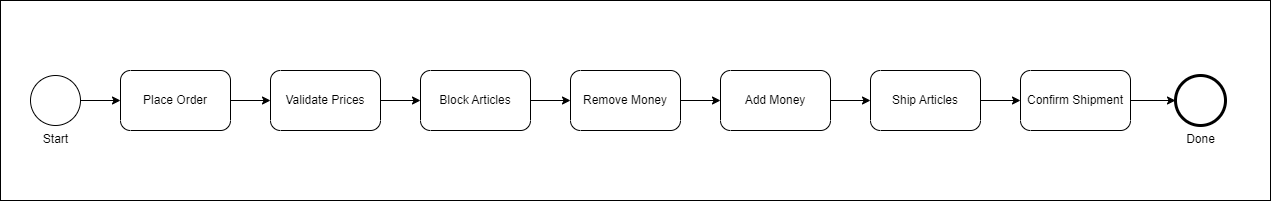
\includegraphics[width=\linewidth]{figures/SimplifiedBusinessProcess.png}
\end{figure}


% TODO Diagramm für den vereinfachten Prozess

Die zum Prozess gehörenden Schritte sind folgende:

\subparagraph*{Entgegennehmen der Bestellung} Die Bestellung wird über ein imaginäres Frontend entgegengenommen. Dieses Frontend baut einen Request auf und sendet diesen per Http-Schnittstelle an das Backend. Dort wird der Request entgegengenommen und muss alle für die Abwicklung der Bestellung erforderlichen Daten enthalten. Dazu gehören der bestellende Nutzer, die geforderten Artikel und die Zahlungsinformationen. Beim Entgegennehmen wird die Bestellung initialisiert.

\subparagraph*{Validierung des Preises} Der Bestellungsrequest enthält eine Liste von den gewünschten Produkten und dem bekannten Preis pro Produkt. Um zu überprüfen, ob der dem Nutzer (dem Frontend) bekannte Preis mit dem aktuellen Preis übereinstimmt, muss dieser validiert werden. % TODO warum ist dieser Schritt notwendig	

\subparagraph*{Blockieren der Artikel} Die geforderten Artikel sollten für diese Bestellung reserviert werden, bis der Bestellvorgang abgeschlossen ist. In einem Online-Shop wird angezeigt, wieviele Artikel auf Lager vorrätig sind. Beim Blockieren der Artikel wird dieser Betrag verändert. Somit sehen andere Nutzer nach Ausführung dieses Schrittes den aktuellen Wert der vorrätigen Artikel. 

\subparagraph*{Zahlungsabwicklung} Der berechnete Preis der Bestellung muss vom Konto des Kunden abgebucht werden. Das Konto des Händlers erhält denselben Betrag gutgeschrieben. Die Konten des Kunden und des Online-Shop-Besitzers müssen nicht bei derselben Bank liegen. 

\subparagraph*{Auslösen der Lieferung} Die blockierten Artikel werden versendet. Dieser Prozess dauert einen längeren Zeitraum an.

\subparagraph*{Abschluss der Lieferung} Der Lieferant bestätigt die Übergabe der Waren an den Kunden.


\paragraph*{Implementierung}

Nachdem der Geschäftsprozess definiert wurde, soll das Saga-System implementiert werden. In \ref{sec_saga_formalisierung_dea} wurde erläutert, wie die im Koordinator laufende SEC beschrieben werden kann. Die Implementierung soll durch diese Darstellungsform beschrieben werden können.

Für die Transaktionsteilnehmer gilt zu Beginn der Implementierung lediglich die Anforderung, dass die Schnittstellen per Request-Response-Muster aufgerufen werden. Dafür wird das Http-Protokoll verwendet.


\subsection{Schritt 2 - Messung der verschiedenen Implementierungen}

Die Bewertung der Implementierungen soll auf Grundlage von Messdaten erfolgen. Es soll nun beschrieben werden, wie die Erfassung dieser Daten erfolgen soll.

% TODO Testpyramide

\paragraph*{Systemtest} \mbox{}\\
Die Messdaten erfolgen in einer produktionsähnlichen Umgebung im Rahmen von Systemtests. Das erwartete Ergebnis ist ein konkreter Endzustand, der erreicht werden soll. Dieser Endzustand kann mit dem erreichten Endzustand verglichen werden.

\paragraph*{Testkonfiguration} \mbox{}\\
Ein solcher Systemtest wird unter einer bestimmten Konfiguration durchgeführt. Die Konfiguration setzt sich zusammen aus einem Testcase und einem Netzwerkszenario. 

\paragraph*{Testcase} \mbox{}\\
Ein Testcase stellt eine konkrete Interaktion mit dem System dar. Die Testcases übernehmen die Aufgabe, die verschiedenen Fälle der Geschäftslogik auf Korrektheit zu überprüfen.

\paragraph*{Netzwerkszenarien} \mbox{}\\
Ein Netzwerkszenario ist ebenfalls Teil der Testkonfiguration. Wird ein Systemtest durchgeführt, so beschreibt das Netzwerkszenario das konkrete Netzwerkverhalten.

% TODO wie misst man Konsistenz
\paragraph*{Messgegenstand} \mbox{}\\
Das Ziel der Messung ist, Aussagen über die Konsistenz des Systems zu treffen. In Abschnitt \ref{} wurden verschiedene Vorgehensweisen dargestellt, wie die Konsistenz eines Systems gemessen werden kann. 

Die verwendete Implementierung per Orchestrierung setzt das Vorhandensein eines Koordinators voraus. Die darin befindliche Steuerung der LLT durch die SEC gibt Auskunft über die ausgeführten lokalen Transaktionen einer Saga. Es kann für jede lokale Transaktion gemessen werden, wie oft die SEC davon ausgeht, dass eine Transaktion ausgeführt wurde. Analog dazu kann die tatsächlich ausgeführte Anzahl an Transaktionen bestimmt werden, indem die Sicht der Transaktionsteilnehmer verwendet wird. Stimmen die korrespondierenden Werte aller lokalen Transaktionen in beiden Sichten überein, kann davon ausgegangen werden, dass die LLT keine Inkonsistenzen in das System eingeführt hat.

Ein weiterer Anhaltspunkt für Konsistenzanomalien ist der erreichte Endzustand einer Transaktion. In \ref{sec_saga_formalisierung_dea} wurde ein Endzustand für einen DEA definiert, der erreicht wird, nachdem eine Saga in einer kompensierenden Aktion eine Fehlerantwort erhält. In solchen Fällen ist der Koordinator nicht in der Lage die LLT abzuschließen und endet in einem weder erfolgreichen noch kompensierten Zustand. 

Da dieser Zustand einen Fall aufzeigt, in dem die Atomarität der LLT verletzt wird, ist das Auftreten solcher Endzustände ein unmittelbares Zeichen für Inkonsistenz.

\paragraph*{Metriken} \mbox{}\\
% TODO
TODO Beschreibung, wie die Messdaten in eine (oder mehrere) Kennzahlen umgewandelt wird
\subsection{Analyse der Messdaten}
Die Ergebnisse aus der Messung stellen die Grundlage für eine Analyse des implementierten Systems dar. Die Messwerte geben Auskunft über Konsistenz, Laufzeit und Erfolgsrate. Die Werte sollen interpretiert werden. Es sind Ursachen für Konsistenzanomalien, übermäßig lange oder unbeendete Ausführungen sowie erfolglose LLTs zu identifizieren. 






%Was mache ich in dem praktischen Teil
%- was ist das ziel?
%	- zusammenhänge zwischen konsistenz und schnittstellendesign erkennen
%	- these beantworten: können Netzwerkpartitionen in Sagapattern einbezogen werden
%- methodik
%	- schritt 1: entwurf+impl eines gp
%		- anforderungen an den Gp definieren
%		- 
%	- schritt 2: durchführung von messungen 
%		- was wird gemessen?
%			- erreichte endzustände (entspricht der Sicht des Koordinators)
%			- ausgeführte Transaktionen aus Sicht des Koordinators und der Teilnehmer	
%		- unter welchen Bedingungen wird gemessen?
%			- Szenario 1, 2, 3
%			- wie werden diese Bedingungen geschaffen
%		- welche Usecases werden für die Messungen durchgeführt
%			- UC 1, 2
%	- schritt 3: 
%		- Analyse der Werte
%		- Schlüsse ziehen








	
	
	\input{texes/ChapterVersuchsdurchführung.tex}
	
	\chapter{Implementierung}

	
	\chapter{Ausblick, Ansatz für weitere Untersuchungen}

\section{asdasdas}
asdasdasd
	
	\pagebreak
	
	\pagenumbering{Roman}
	\listoffigures
	\addcontentsline{toc}{chapter}{Abbildungsverzeichnis}
	
	\printnoidxglossaries
	\addcontentsline{toc}{chapter}{Akronyme}
	
	\printbibliography
	\addcontentsline{toc}{chapter}{Literaturverzeichnis}
	
	\pagebreak
	%\input{texes/Selbstständigkeitserklärung.tex}
\end{document}